\documentclass{article}

\textwidth=6.5in
\textheight=8.5in
\voffset=-54pt
\oddsidemargin=0in
\evensidemargin=0in
\setlength{\parskip}{8pt}
\setlength{\parindent}{0pt}

\usepackage{amsmath, amssymb}
\usepackage{ifthen}

\usepackage[inline]{enumitem}
\setlist{topsep=0pt, parsep=8pt}

\usepackage[rgb,table]{xcolor}\convertcolorsUfalse
\usepackage{graphicx}

% change hyperref options
\PassOptionsToPackage{hyphens}{url}
\usepackage[bookmarks,colorlinks,linkcolor=black,citecolor=blue,pdfstartview=FitH,urlcolor=blue]{hyperref}
\hypersetup{pdfpagemode=UseNone}
\usepackage{bookmark}

\usepackage{graphicx}
\usepackage{multicol}
\usepackage{framed}
\usepackage{array}

\usepackage{icomma}

\usepackage{pifont}

\usepackage{marginnote}
\usepackage[colorinlistoftodos]{todonotes}
\renewcommand{\marginpar}{\marginnote}

\usepackage{soul}

\usepackage{pgfplots}
\pgfplotsset{compat=1.18}  
\pgfplotscreateplotcyclelist{mycolor}{black, blue, red, green!70!black, magenta, purple, cyan, orange }  
\pgfplotsset{
  disabledatascaling,
  cycle list=tikzcolor, 
  axis lines=middle,
  every axis plot/.style={no marks, thick},
  every axis/.style={
    enlarge x limits=false,
    enlarge y limits=auto,
    xlabel style={at={(current axis.right of origin)},anchor=west},
    ylabel style={at={(current axis.above origin)},anchor=south},
    % extra x and y ticks for asymptotes
    extra x tick style={grid=major, grid style={dashed,black}},
    extra y tick style={grid=major, grid style={dashed,black}},
    /pgf/number format/1000 sep={},
  },    
  tick label style = {font=\footnotesize, fill=\currentbgcolor, inner sep=0pt},    
  xticklabel shift=1pt,    
  scaled ticks=false,
  scaled y ticks=false,
  unbounded coords=jump,
  samples=101,
  minor tick length=0,
  scatter/classes={
    open={mark=*,draw=black,fill=white, mark size=2, thin},
    closed={mark=*,draw=black,fill=black, mark size=2, thin}
  },
  width=3in,
}
\pgfplotsset{open/.style={only marks, mark=*, fill=white, thin, mark size=2}}
\pgfplotsset{closed/.style={only marks, mark=*, draw=black, fill=black,
    thin, mark size=2}}
\pgfplotsset{labeled/.style={nodes near coords, only marks, mark=*, draw=black, fill=black, thin, mark size=2, point meta=explicit symbolic}}

\pgfplotsset{gridgraph/.style={clip=false, axis line style={shorten
      >=-8pt}, xlabel style={xshift=8pt}, ylabel style={yshift=8pt},
    enlargelimits=false, grid=major, tick style={black}}} 

\newcommand{\axes}[1][]{
  \begin{tikzpicture}
    \begin{axis}[xtick=\empty, ytick=\empty, ymin=-2, ymax=2,
      xmin=-4.25, xmax=4.25, #1]
    \end{axis}
  \end{tikzpicture}
}

\usepackage{tikz}
\usetikzlibrary{
  matrix,%
  % enables the snake paths
  decorations.pathmorphing,%
  % enables bigger arrows
  decorations.markings,%
  decorations.pathreplacing,%
  decorations.text,%
  calc,%
  patterns,%
  shapes.geometric,%
  arrows,
  decorations.shapes,
  positioning,
  plotmarks,
  intersections
}
\tikzset{>=latex} % sets default arrow type in tikz
\tikzset{font=\normalsize}
\tikzset{mark size=1.5pt, mark options=thin}
\tikzset{pin distance=4pt,
  every pin edge/.style={<-, thin, shorten <= -2pt}}

\interfootnotelinepenalty=10000
\renewcommand{\thefootnote}{(\arabic{footnote})}

\usepackage{multirow, bigdelim}

% change to \usepackage[sols]{handout} to see solutions
\usepackage[]{handout}

\providecommand{\check}{}
\renewcommand{\check}{\ifmmode{\text{ \ding{51} }}\else{\ding{51} }\fi}

\newcommand\iscurrentenumi[1]{%
  \ifthenelse{\equal{#1}{\theenumi}}{}{#1}}
\setenumerate[1]{ref=\#\arabic*}
\setenumerate[2]{ref=\protect\iscurrentenumi{\theenumi}(\alph*)}
\newcommand\enumiiprefix[2]{%
  \ifthenelse{{\equal{#1}{\theenumi}}\AND{\equal{#2}{(\alph{enumii})}}}{}{}%
  \ifthenelse{{\equal{#1}{\theenumi}}\AND{\NOT{\equal{#2}{(\alph{enumii})}}}}{#2}{}%
  \ifthenelse{\equal{#1}{\theenumi}}{}{#1#2}%
}
\setenumerate[3]{ref=\protect\enumiiprefix{\theenumi}{(\alph{enumii})}\roman*}

\newlength{\tipmargin}
\makeatletter

\renewenvironment{framed}{
  \setlength{\tipmargin}{\textwidth-\linewidth}
  \advance\@totalleftmargin-\tipmargin
  \def\FrameCommand{\hspace{\tipmargin}\fbox}%
  \advance\linewidth\tipmargin
  \MakeFramed {\advance\hsize-\width \FrameRestore}%
}
{\endMakeFramed}

\makeatother

\definecolor{purple}{rgb}{0.5,0,1.0}

\usepackage{fancyhdr}
\lhead{\textcolor{white}{This content is protected and may not be shared, uploaded, or distributed.}}
\rhead{}
\rfoot{\vspace*{\fill}\footnotesize\textcopyright{} \emph{Harvard Math Ma}}
\renewcommand{\headrulewidth}{0pt}
\pagestyle{fancy}
\begin{document}

\htitle{30. Logarithm Rules}

\begin{problemonly}
  \begin{framed}

You should be able to:
    \begin{itemize}[topsep=0pt,partopsep=0pt,parsep=8pt,itemsep=0pt]

    \item Apply basic properties of logarithms. (Can we simplify the log of a product? How about the log of a sum, quotient, or power?) 

    \item Change bases of logarithms (for example, rewrite $\log_2 3$ in terms of $\ln$ or $\log_7$). 

    \end{itemize}
  \end{framed}
\end{problemonly}

\begin{enumerate}
\item 

  \note{This is a warm up. Nothing here is new, but it's a chance to catch errors students are making. I'll probably do the first two parts with them, just to get them thinking in the right direction, and then have them try the rest.}

  Simplify each as much as possible. (An expression might already be simplified, or it might be undefined, so be careful!)

  \begin{enumerate}
  \item
    \begin{problem}
      $\displaystyle \log_5 25 = \fitb{0.25in}{}$ because 
    \end{problem}

    \begin{solution}
      $\boxed{2}$, since $5^2 = 25$.
    \end{solution}

  \item
    \begin{problem}
      $\displaystyle \ln \left( e \sqrt{e} \right) = \fitb{0.25in}{}$ because
    \end{problem}

    \begin{solution}
      $\boxed{\frac{3}{2}}$, since $e^{3/2} = e\sqrt{e}$.
    \end{solution}

  \item
    \begin{problem}
      $\displaystyle \ln \left( \frac{1}{e \sqrt{e}} \right) = \fitb{0.25in}{}$ because 
    \end{problem}

    \begin{solution}
      $\boxed{-\frac{3}{2}}$, since $e^{-3/2} = \frac{1}{e \sqrt{e}}$. 
    \end{solution}

  \item
    \begin{problem}[\vfill]
      $\displaystyle 11^{\log_5 11}$
    \end{problem}

    \begin{solution}
      We can't simplify this any further.
    \end{solution}

  \item
    \begin{problem}[\vfill]
      $\displaystyle 7^{\log_7 3}$
    \end{problem}

    \begin{solution}
      $\boxed{3}$, using the rule that 
      $7^{\log_7 \heartsuit} = \heartsuit$.
    \end{solution}

  \item

    \begin{problem}[\vfill]
      $\displaystyle e^{-3 \ln 2}$
    \end{problem}

    \begin{solution}
      $\boxed{\frac{1}{8}}$, since $e^{-3 \ln 2}=(e^{\ln2})^-3$.

    \end{solution}

  \item

    \begin{problem}[\vfill]
      $\displaystyle \log_3 \left( 3^5 \cdot 3^8 \right)$
    \end{problem}

    \begin{solution}
      $\boxed{13}$, since 
      $\log_3 ( 3^5 \cdot 3^8 )= \log_3 (3^{13})$.
    \end{solution}

  \item
    \begin{problem}[\vfill]
      $\log_{10} \left( 10^2 - 10^3 \right)$
    \end{problem}

    \begin{solution}
      We can't simplify this any further.
    \end{solution}

  \item

    \begin{problem}[\vfill\newpage]
      $\displaystyle \log_2 \left( \frac{2^{11}}{2^6} \right)$
    \end{problem}

    \begin{solution}
      Since $\frac{2^6}{2^{11}} = 2^{-5}$, this is equal to
      $\log_2 \left( 2^{-5} \right) = \boxed{-5}$.
    \end{solution}

  \end{enumerate}

\item  \label{log-rules-idea}

  \note{These are meant to help students come up with the log rules. We'll do the first part together because I don't want students who have seen log rules before to try to blindly apply them.

    Here's the type of reasoning I'd like them to use: We're told that $\log_3 4 \approx 1.26$ and $\log_3 7 \approx 1.77$, which is the same as saying $3^{1.26} \approx 4$ and $3^{1.77} \approx 7$. Therefore, $\dfrac{7}{4} \approx \dfrac{3^{1.77}}{3^{1.26}} = 3^{1.77 - 1.26}$, so $\log_3 \left( \dfrac{7}{4} \right) \approx 1.77 - 1.26 = \log_3 7 - \log_3 4$. }

  Here are two facts: $\log_3 4 \approx 1.26$ and $\log_3 7 \approx 1.77$. We'll use these two facts to help you approximate the following quantities, and explain your reasoning in each.

  \begin{enumerate}
  \item 
    \begin{problem}[\vfill]
    Rewrite $\log_3 4 \approx 1.26$ and $\log_3 7 \approx 1.77$ as relationships between quantities that involve exponential functions.
    \end{problem}
    \begin{solution}
        $3^{1.26} \approx 4$ and $3^{1.77}\approx 7$
    \end{solution}
  \item
    \begin{problem}
      By substituting these expressions for 7 and 4, simplify the following: 
      \end{problem}
      \begin{enumerate}
          \item 
          \begin{problem}[\vfill]
          $\log_3 \left( \dfrac{7}{4} \right)$
          \end{problem}
    \begin{solution}      
      We're told that $\log_3 4 \approx 1.26$ and
  $\log_3 7 \approx 1.77$, which is the same as saying $3^{1.26} \approx 4$ and $3^{1.77} \approx 7$. Therefore, $\dfrac{7}{4} \approx \frac{3^{1.77}}{3^{1.26}} = 3^{1.77 - 1.26}$, so $\log_3 \left( \dfrac{7}{4} \right) \approx 1.77 - 1.26$. 
    \end{solution}

  \item
    \begin{problem}[\vfill]
      $\log_3 28$
    \end{problem}

    \begin{solution}
      Using the same idea as before,
      we can rewrite $28=4\times 7$ as approximately
      $3^{1.26} \times 3^{1.77}$, 
      which is $3^{1.26+1.77}$, so $\log_3(28) \approx 1.26 + 1.77$.
    \end{solution}

  \item
    \begin{problem}[\vfill]
      $\log_3 \left( 7^{2.1} \right)$
    \end{problem}

    \begin{solution}
      Since $7 \approx 3^{1.77}$, we can rewrite $7^{2.1}$ as approximately
      $(3^{1.77})^{2.1}$, or $3^{2.1\times1.77}$. This means that
      $\log_3\left(7^{2.1}\right) \approx 2.1 \times 1.77$.
    \end{solution}
\end{enumerate}
  \end{enumerate}

\end{enumerate}
Generalize the rules from the previous problem:

\begin{framed}
  \textbf{Logarithm Rules.}  
  \begin{enumerate}[topsep=0pt]
  \item \solonly{$\displaystyle \log_b (uw) = \log_b u + \log_b w$} \

    \bigskip

  \item \solonly{$\displaystyle \log_b \left( \frac{u}{w} \right) = \log_b u - \log_b w$}\

    \bigskip

  \item \solonly{$\displaystyle \log_b \left( u^n \right) = n \log_b u$}\

    \bigskip

  \end{enumerate}  
\end{framed}

\begin{enumerate}[resume]
\item 

  \note{I want students to see that they can easily come up with an example if they ever forget this. For example, $\log_{10}(10) = 1$ and $\log_{10} (100) = 2$, but $\log_{10}(10 + 100)$ isn't a nice number.}

  \begin{problem}[\vfill\newpage]
    Is there a nice rule for taking $\log_b$ of a sum? Come up with a convincing example to support your answer. 
  \end{problem}

  \begin{solution}
    No, there is no nice rule for the logarithm of a sum. For example,
    For example, $\log_{10}(10) = 1$ and $\log_{10} (100) = 2$, but 
    $\log_{10}(10 + 100)$ isn't a nice number.
  \end{solution}

\end{enumerate}
\note{The next few problems are practice applying the log rules; we probably won't do all of them because I want to make sure there's time for the change of base formula. So, at some point, I will have students move on to \ref{log-graphs}.}

\begin{enumerate}[resume]
\item 

  \begin{enumerate}
  \item
    \begin{problem}[\vfill]
      Express $\ln(w u^2)$ in terms of $A = \ln u$ and $B = \ln w$. (Begin by rewriting the relationship between the variables using exponential functions. Which base should you use?)
    \end{problem}

    \begin{solution}
      \begin{align*}
        \ln \left( u^2 w \right) &= \ln \left( u^2 \right) + \ln w \\
        &= 2 \ln u + \ln w \\
        &= \boxed{2A + B}
      \end{align*}
    \end{solution}

  \item
    \begin{problem}[\vfill]
      Express $\ln \left[ (wu)^2 \right]$ in terms of $A = \ln u$ and $B = \ln w$. Is this the same as or different from (a)?
    \end{problem}

    \begin{solution}
    \begin{align*}
          \ln \left[ (wu)^2 \right] &= 2\ln\left(uw\right) \\
          &= 2(\ln u + \ln w )\\
          &= \boxed{2(A + B)}
      \end{align*}
      Alternatively,
      \begin{align*}
          \ln \left[ (wu)^2 \right] &= \ln\left(u^2 w^2\right) \\
          &= \ln(u^2) + \ln (w^2) \\
          &= 2\ln u + 2\ln w \\
          &= 2A + 2B.
      \end{align*}
      We can see that this is different from our answer to part (a).
    \end{solution}

  \end{enumerate}

\item  If possible, simplify each expression, and write it in terms of $A =
  \log_2 u$ and $B = \log_2 w$ (with no logarithms in your final answer). 

  \begin{enumerate}
  \item

    \note{I expect lots of parentheses errors here.}

    \begin{problem}[\vfill]
      $\displaystyle 7 \log_2 \left( \frac{8}{\sqrt{uw}}\right)$
    \end{problem}

    \begin{solution}
      \begin{align*}
        7\log_2 \left( \frac{2}{\sqrt{uw}}\right) &= 7\left[ \log_2 8 - \log_2\!
          \sqrt{uw} \right] \\
        &= 7\left[3 - \frac{1}{2} \log_2 uw \right] \\
        &= 7\left[3 - \frac{1}{2} \left( \log_2 u + \log_2 w \right)\right] \\
        &= 7\left[3 - \frac{1}{2} \log_2 u - \frac{1}{2} \log_2 w\right] \\
        &= \boxed{7\left(3 - \frac{1}{2} A - \frac{1}{2} B\right)}
      \end{align*}
    \end{solution}

  \item
    \begin{problem}[\vfill]
      $7 \log_2 \left( u + \sqrt{8w} \right)$
    \end{problem}

    \begin{solution}
      We don't have any way of simplifying the log of a sum.
    \end{solution}

  \item 
    \begin{problem}[\vfill\newpage]
      $\displaystyle 7 \log_2 \left( \frac{8}{\sqrt{u} w}\right)$. Is this the same as or different from (a)?
    \end{problem}

    \begin{solution}
      \begin{align*}
        7\log_2 \left( \frac{2}{\sqrt{u}w}\right) &= 7\left[ \log_2 8 - \log_2\! \left(
          \sqrt{u}w \right)\right] \\
        &= 7\left[ \log_2 8 - \left(\log_2\!
          \sqrt{u} + \log_2 w\right) \right] \\
          &= 7\left[ \log_2 8 - \log_2\!
          \sqrt{u} - \log_2 w \right] \\
        &= 7\left[3 - \frac{1}{2} \log_2 u - \log_2 v\right] \\
        &= \boxed{7\left(3 - \frac{1}{2} A - B\right)}
      \end{align*}
      This is not the same as our answer to (a).
    \end{solution}

  \end{enumerate}

\item  Simplify the following, if possible:

  \probonly{\begin{multicols}{3}}
    \begin{enumerate}

    \item $\displaystyle \ln(7^3) - \ln(7)$

    \begin{solution}
        $\ln(7^3) - \ln(7) = 3\ln (7)-\ln (7) = 2\ln 7$
    \end{solution}

    \item $\displaystyle \left( \log_3 7 \right) \left( \log_3 8 \right)$

    \begin{solution}
      There's nothing we can do to simplify this.
    \end{solution}

    \item
      $\displaystyle \log_8 (x+1) + \log_8 \left( \frac{1}{x+1} \right)$

    \begin{solution}
        $\displaystyle \log_8 (x+1) + \log_8 \left( \frac{1}{x+1} \right)
        = \log_8\left(\frac{x+1}{x+1}\right) = \log_8 1 = 0$
    \end{solution}

    \end{enumerate}
  \probonly{\end{multicols}}

  \pspace{\stretch{0.35}}

\item  \label{log-graphs}

  \note{Students will hopefully remember the general shape of these graphs, but they may have trouble with the relative placement. I will encourage them to reason it out by thinking about how $2^x$, $e^x$, and $3^x$ relate (testing points if necessary).}

  \begin{problem}[\stretch{1.5}]
    On the same set of axes, graph $\ln x$, $\log_2 x$, and $\log_3 x$ in 3 different colors. (What's our usual strategy for graphing a log?) Where are the asymptotes and intercepts of each graph? 
  \end{problem}

  \begin{solution}
    \begin{center}
      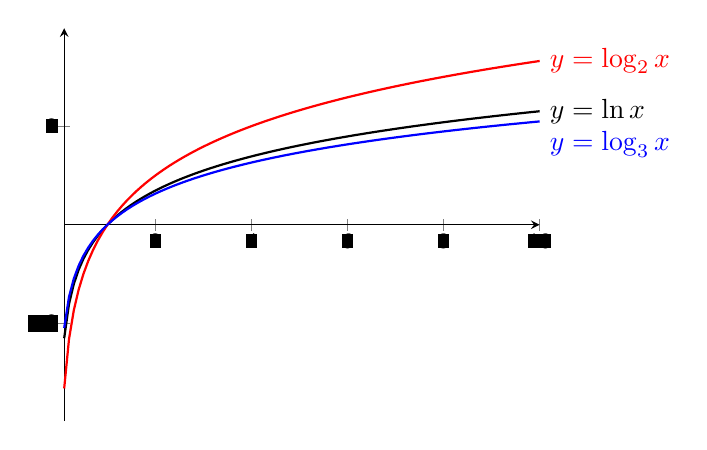
\begin{tikzpicture}
        \begin{axis}[clip=false]
          \addplot[domain=0:10, black] {ln(x)} 
            node[right] {$y=\ln x$};
          \addplot[domain=0:10, red] {ln(x)/ln(2)} 
            node[right] {$y=\log_2 x$};
          \addplot[domain=0:10, blue] {ln(x)/ln(3)} 
            node[below right] {$y=\log_3 x$};
        \end{axis}
      \end{tikzpicture}
    \end{center}
    All of the graphs have an $x$-intercept at $(1,0)$, and they
    all have a vertical asymptote of $x=0$.
  \end{solution}

\item  \label{log-base-b-in-terms-of-ln-example}

  \begin{problem}[\vfill]
    Rewrite $\log_5 17$ in terms of natural logs.  (Strategy: Give $\log_5
    17$ a name like $x$, rewrite the equation $x = \log_5 17$ as an
    equation involving exponents, and then take the natural log of both
    sides and solve for $x$.)
  \end{problem}

  \begin{solution}
    Let $x = \log_5 17$. Then,
    \begin{align*}
      5^x &= 17 \\
      \intertext{Taking ln of both sides,}
      \ln \left( 5^x \right) &= \ln 17 \\
      x \ln 5 &= \ln 17 \\
      x &= \boxed{\frac{\ln 17}{\ln 5}}
    \end{align*}
  \end{solution}

\end{enumerate}
\begin{framed}  
  \emph{\bf Change of base to natural log}: \probonly{$\vphantom{\boxed{\int_1^2}}$}$\log_b a = \solonly{\dfrac{\ln a}{\ln b}}$
\end{framed}

\begin{enumerate}[resume, topsep=0pt]

\item 

  \note{Now, we can see from the change of base formula that $\log_2 x$ and $\log_3 x$ are both vertical stretches of $\ln x$.} 

  \begin{problem}[\nstretch{0.75}]
    Explain how the change of base formula is consistent with your graphs in \ref{log-graphs}.
  \end{problem}

  \begin{solution}
    Using the change of base formula, $\log_2{x} = \dfrac{\ln x}{\ln 2}$,
    and $\log_3 {x} = \dfrac{\ln x}{\ln 3}$, so they are just $\ln x$
    divided by constants. This is consistent
    with our graphs, which show that 
    $y=\log_2 x$ and $y=\log_3 x$ are vertically scaled copies of 
    $y=\ln x$.
  \end{solution}

  \pspace{\newpage}

\item  
  \begin{problem}[2.5in]
    Graph $f(x) = \displaystyle \log_3 \left( \frac{9}{x^2} \right) +
    \log_3 x$.  (\textit{Hint:} First use log rules to simplify.)  Label
    all intercepts and asymptotes, and label at least two other points on
    the graph with exact coordinates.
  \end{problem}

  \begin{solution}
    \begin{align*}
      f(x) &= \log_3 \left( \frac{9}{x^2} \right) + \log_3 x \\
      &= \log_3 9 - \log_3 (x^2) + \log_3 x \\
      &= 2 - 2 \log_3 x + \log_3 x \\
      &= 2 - \log_3 x
    \end{align*}

    There is a vertical asymptote at $x=0$. There are no $y$-intercepts.
    To find the $x$-intercept, we set $f(x)=0$ and solve for $x$.
    \begin{align*}
        2 - \log_3 x &= 0 \\
        \log_3 x &= 2 \\
        x &= 9
    \end{align*}

    \begin{center}
      \begin{tikzpicture}
        \begin{axis}[xtick={1,3,9}, ytick={1,2}]
          \addplot[domain=0:10] {2-ln(x)/ln(3)};
          \addplot[closed] coordinates {(1,2) (3,1)};
        \end{axis}
      \end{tikzpicture}
    \end{center}
  \end{solution}

\item 
  \begin{enumerate}
  \item
    \begin{problem}[\vfill]
      Simplify $\log_8 32$. (\emph{Hint:} If you're having trouble, try using the strategy of \ref{log-base-b-in-terms-of-ln-example} to rewrite this in terms of base 2 logarithms.)
    \end{problem}

    \begin{solution}
      Let $y=\log_8 32$. Then $8^y = 32$. Using the hint,
      if we take the logarithm base 2 of both sides, then
      \begin{align*}
          8^y &= 32\\
          \log_2 (8^y) &= \log_2 32 \\
          y \log_2 8 &= \log_2 32 \\
          y &= \frac{\log_2 32}{\log_2 8} \\
          y &= \boxed{\frac{5}{3}}.
      \end{align*}
      This also shows us that we can use the change of base formula
      to change to any base.
    \end{solution}
    

  \item
    \begin{problem}[0.5in]
      \check How can you check your answer?
    \end{problem}

    \begin{solution}
      We can check that $8^{5/3} = (\sqrt[3]{8})^5 = 32$.
    \end{solution}
  \end{enumerate}

\item 
  \begin{problem}[\stretch{0.5}]
    Can you use exponent rules to simplify $e^{4 \ln 3}$? Can you use log rules to simplify $e^{4 \ln 3}$? 
  \end{problem}

  \begin{solution}
    Using exponent rules, $e^{4\ln3} = (e^{\ln3})^4 = 3^4=81$.

    Using log rules, $e^{4\ln3} = e^{\ln(3^4)} = 3^4 = 81$. 
  \end{solution}

\end{enumerate}
\end{document}
